\ifx\wholebook\relax \else

\documentclass{article}

%
% loading packages
%

\RequirePackage{ifpdf}
\RequirePackage{ifxetex}

%
%
\ifpdf
  \RequirePackage[pdftex,%
       bookmarksnumbered,%
              colorlinks,%
          linkcolor=blue,%
              hyperindex,%
        plainpages=false,%
       pdfstartview=FitH]{hyperref}
\else\ifxetex
  \RequirePackage[bookmarksnumbered,%
               colorlinks,%
           linkcolor=blue,%
               hyperindex,%
         plainpages=false,%
        pdfstartview=FitH]{hyperref}
\else
  \RequirePackage[dvipdfm,%
        bookmarksnumbered,%
               colorlinks,%
           linkcolor=blue,%
               hyperindex,%
         plainpages=false,%
        pdfstartview=FitH]{hyperref}
\fi\fi
%\usepackage{hyperref}

% other packages
%--------------------------------------------------------------------------
\usepackage{graphicx, color}
\usepackage{wrapfig}
\usepackage{subfig}
\usepackage{multicol}
\usepackage{tikz}
\usetikzlibrary{matrix,positioning,shapes}
\usetikzlibrary{patterns}

\usepackage{amsmath, amsthm, amssymb} % for math
\usepackage{exercise} % for exercise
\usepackage{import} % for nested input

%
% for programming
%
\usepackage{verbatim}
\usepackage{fancyvrb}
\usepackage{listings}
%\usepackage{algorithmic} %old version; we can use algorithmicx instead
%\usepackage[plain]{algorithm} %remove rule (horizontal line on top/below the algorithm
\usepackage{algorithm} %to remove rules change to \usepackage[plain]{algorithm}
%\usepackage{algorithm2e}
\usepackage[noend]{algpseudocode} %for pseudo code, include algorithmicsx automatically
\usepackage{appendix}
\usepackage{makeidx} % for index support
\usepackage{titlesec}
\usepackage{epigraph}

\usepackage[cm-default]{fontspec}
\usepackage{xunicode}
%\usepackage{fontenc}
\usepackage{textcomp}
\usepackage{url}

% detect and select Chinese font
% ------------------------------
% fc-list :lang=zh    % list all Chinese fonts
% fc-list :mono       % list all mono fonts
% fc-cache            % refresh cache to load new installed fonts
\def\macmainfont{STSong}  % Under Mac OS X
\def\macmonofont{Monaco}
\def\winmainfont{SimSun} % Under Windows
\def\winmonofont{Consolas}
\def\linuxmainfont{WenQuanYi Micro Hei} % Under Linux
\def\linuxmainfont{Courier}

\suppressfontnotfounderror1 % Avoid setting exit code (error level) to break make process
\count255=\interactionmode
\batchmode

% main font
\let\mainft=\macmainfont
\font\thefont="\mainft"\space at 10pt
\ifx\thefont\nullfont
  \let\mainft=\winmainfont
  \font\thefont="\mainft"\space at 10pt
  \ifx\the\nullfont
    \let\mainft=\linuxmainfont
    \font\thefont="\mainft"\space at 10pt
    \ifx\the\nullfont
      \errorstopmode
      \errmessage{no suitable Chinese main font found}
    \fi
  \fi
\fi

% mono font
\let\monoft=\macmonofont
\font\thefont="\monoft"\space at 10pt
\ifx\thefont\nullfont
  \let\monoft=\winmonofont
  \font\thefont="\monoft"\space at 10pt
  \ifx\the\nullfont
    \let\monoft=\linuxmonofont
    \font\thefont="\monoft"\space at 10pt
    \ifx\the\nullfont
      \errorstopmode
      \errmessage{no suitable mono font found}
    \fi
  \fi
\fi

\interactionmode=\count255

\setmainfont[Mapping=tex-text]{\mainft}
\setmonofont[Scale=MatchLowercase]{\monoft}   % 英文等宽字体

\XeTeXlinebreaklocale "zh"  % to solve the line breaking issue
\XeTeXlinebreakskip = 0pt plus 1pt minus 0.1pt

\titleformat{\paragraph}
{\normalfont\normalsize\bfseries}{\theparagraph}{1em}{}
\titlespacing*{\paragraph}
{0pt}{3.25ex plus 1ex minus .2ex}{1.5ex plus .2ex}

\lstdefinelanguage{Smalltalk}{
  morekeywords={self,super,true,false,nil,thisContext}, % This is overkill
  morestring=[d]',
  morecomment=[s]{"}{"},
  alsoletter={\#:},
  escapechar={!},
  literate=
    {BANG}{!}1
    {UNDERSCORE}{\_}1
    {\\st}{Smalltalk}9 % convenience -- in case \st occurs in code
    % {'}{{\textquotesingle}}1 % replaced by upquote=true in \lstset
    {_}{{$\leftarrow$}}1
    {>>>}{{\sep}}1
    {^}{{$\uparrow$}}1
    {~}{{$\sim$}}1
    {-}{{\sf -\hspace{-0.13em}-}}1  % the goal is to make - the same width as +
    %{+}{\raisebox{0.08ex}{+}}1		% and to raise + off the baseline to match -
    {-->}{{\quad$\longrightarrow$\quad}}3
	, % Don't forget the comma at the end!
  tabsize=2
}[keywords,comments,strings]

% for literate Haskell code
\lstdefinestyle{Haskell}{
  flexiblecolumns=false,
  basewidth={0.5em,0.45em},
  morecomment=[l]--,
  literate={+}{{$+$}}1 {/}{{$/$}}1 {*}{{$*$}}1 {=}{{$=$}}1
           {>}{{$>$}}1 {<}{{$<$}}1 {\\}{{$\lambda$}}1
           {\\\\}{{\char`\\\char`\\}}1
           {->}{{$\rightarrow$}}2 {>=}{{$\geq$}}2 {<-}{{$\leftarrow$}}2
           {<=}{{$\leq$}}2 {=>}{{$\Rightarrow$}}2
           {\ .}{{$\circ$}}2 {\ .\ }{{$\circ$}}2
           {>>}{{>>}}2 {>>=}{{>>=}}2
           {|}{{$\mid$}}1
}

% "define" Scala
\lstdefinelanguage{Scala}{
  morekeywords={abstract,case,catch,class,def,%
    do,else,extends,false,final,finally,%
    for,if,implicit,import,match,mixin,%
    new,null,object,override,package,%
    private,protected,requires,return,sealed,%
    super,this,throw,trait,true,try,%
    type,val,var,while,with,yield},
  otherkeywords={=>,<-,<\%,<:,>:,\#,@},
  sensitive=true,
  morecomment=[l]{//},
  morecomment=[n]{/*}{*/},
  morestring=[b]",
  morestring=[b]',
  morestring=[b]"""
}

\lstloadlanguages{C, C++, Java, Lisp, Haskell, Python, Smalltalk, Scala}

\lstset{
  basicstyle=\small\ttfamily,
  commentstyle=\rmfamily,
  texcl=true,
  showstringspaces = false,
  upquote=true,
  flexiblecolumns=false
}

\newcommand\doubleplus{+\kern-1.3ex+\kern0.8ex}

% ======================================================================

\def\BibTeX{{\rm B\kern-.05em{\sc i\kern-.025em b}\kern-.08em
    T\kern-.1667em\lower.7ex\hbox{E}\kern-.125emX}}

%
% mathematics
%
\newcommand{\be}{\begin{equation}}
\newcommand{\ee}{\end{equation}}
\newcommand{\bmat}[1]{\left( \begin{array}{#1} }
\newcommand{\emat}{\end{array} \right) }
\newcommand{\VEC}[1]{\mbox{\boldmath $#1$}}

% numbered equation array
\newcommand{\bea}{\begin{eqnarray}}
\newcommand{\eea}{\end{eqnarray}}

% equation array not numbered
\newcommand{\bean}{\begin{eqnarray*}}
\newcommand{\eean}{\end{eqnarray*}}

\newtheorem{theorem}{定理}[section]
\newtheorem{lemma}[theorem]{引理}
\newtheorem{proposition}[theorem]{Proposition}
\newtheorem{corollary}[theorem]{Corollary}

% 中文书籍设置
% ====================================
\renewcommand\contentsname{目\ 录}
%\renewcommand\listfigurename{插图目录}
%\renewcommand\listtablename{表格目录}
\renewcommand\figurename{图}
\renewcommand\tablename{表}
\renewcommand\proofname{证明}
\renewcommand\ExerciseName{练习}
%\renewcommand{\algorithmcfname}{算法}

\ifx\wholebook\relax
\renewcommand\bibname{参\ 考\ 文\ 献}                    %book类型
%\newtheorem{Definition}[Theorem]{定义}
\newtheorem{Theorem}{定理}[chapter]
\newtheorem{example}{例题}[chapter]
\else
\renewcommand\refname{参\ 考\ 文\ 献}
\fi

%\setcounter{secnumdepth}{4}
\titleformat{\chapter}
  {\normalfont\bfseries\Large}
  {第\arabic{chapter}章}
  {12pt}{\Large}
%% \titleformat{\subsection}
%%   {\normalfont\bfseries\large}
%%   {\CJKnumber{\arabic{subsection}}、}
%%   {12pt}{\large}
%% \titleformat{\subsubsection}
%%   {\normalfont\bfseries\normalsize}
%%   {\arabic{subsubsection}.}
%%   {12pt}{\normalsize}

%\renewcommand{\baselinestretch}{1.5}                        %文章行间距为1.5倍。

\makeatletter
\newcommand{\verbatimfont}[1]{\renewcommand{\verbatim@font}{\ttfamily#1}}
\makeatother

\setcounter{tocdepth}{4}
\setcounter{secnumdepth}{4}

%\verbatimfont{\footnotesize}


\setcounter{page}{1}

\begin{document}

\title{范畴论}

\author{刘新宇
\thanks{{\bfseries 刘新宇} \newline
  Email: liuxinyu95@gmail.com \newline}
  }

\maketitle
\fi

\markboth{范畴论}{编程的数学原理}

\ifx\wholebook\relax
\chapter{范畴论}
\numberwithin{Exercise}{chapter}
\fi

\epigraph{数学是赋予不同事物相同名字的艺术。}{——昂利$\cdot$庞加莱}

% Mathematics is the art of giving the same name to different things.

如果你已经坚持看到了本书这一章,我建议你小小的奖励自己一下。你已经迈过了第一道门槛,正在通往神奇的抽象王国之路上。这条路是世界上许多最聪明的心智披荆斩棘开辟出来的。如果说,人们将具体的事物,抽象成不带具体意义的数与形是原始阶段;将数、形与计算的意义去除,抽象成代数结构(例如群)和代数关系(例如同构)是第一阶段;范畴论可以算是抽象的第二阶段。

你也许会问,我们为什么要了解范畴论?这和编程有什么关系?对此有一个比较短的答案和一个比较长的答案。较短的回答是,如果不了解范畴论,过不了多久,你也许看不懂别人写的程序了。2010年以后,如果翻看Haskell标准库的源代码,就会发现几乎所有的内容,都用范畴论重新写过了。映射、叠加、遍历……几乎所有的计算都在说着范畴的语言,犹如天书。你也许觉得叠加操作可以这样写:

\lstset{language=Haskell, frame=single}
 \begin{lstlisting}
foldr _ z [] = z
foldr f z (x:xs) = f x (foldr f z xs)
\end{lstlisting}

实际上,今天的标准库用范畴的语言这样写:

\begin{lstlisting}
foldr f z t = appEndo (foldMap (Endo #. f) t) z
foldMap f = foldr (mappend . f) mempty
\end{lstlisting}

你也许觉得,反正工作中不用Haskell,不了解范畴论也没有关系。但是最近十几年的情况是,范畴论由于其强大的抽象,几乎普适于任何问题,正向其他的语言和环境中渗透。不要说各大编程语言纷纷引入lambda演算和闭包等结构,有超过20种语言已经实现了单子\cite{Monad-Haskell-Wiki}——用范畴论的语言说,叫做“函子范畴上的幺半群”。

较长的答案是:我们需要抽象。请原谅这个答案看起来更短。赫尔曼$\cdot$外尔说现代数学在过去几十年不断沉湎在抽象和形式化上。编程领域何尝不是如此呢?现代计算机科学解决的问题空前复杂,大数据量、分布式、高并发、还要保证数据和计算的安全。仅仅靠着前几十年的传统方法——暴力求解、务实的工程实践再加上一点聪明的头脑已经不够了。这逼迫着我们去吸取其他科学和数学中的新方法和新工具。

正如迪厄多内所说:“这种抽象绝不是来自数学家的反常意愿,似乎他们想通过使用深奥莫测的语言来把自己与其它人隔开。数学家是被经典对象和关系的本质特性逼着去锻造新的抽象工具,来解决过去看来是不可攻克的问题。”\cite{Dieudonne1987}

本章内容将再次挑战我们的抽象思维。如果读完一遍没有理解是完全正常的。请不要灰心丧气,生活不是直线发展的,我们理解知识的过程是螺旋上升的。要不断回过头去反复体会。开卷有益,去阅读大师的作品。也许某个瞬间豁然开朗,就能体会到“蓦然回首,那人却在灯火阑珊处”的感觉。

范畴论是数学家艾伦伯格和麦克兰恩在1940年代创立的。

\begin{wrapfigure}{R}{0.3\textwidth}
 \centering
 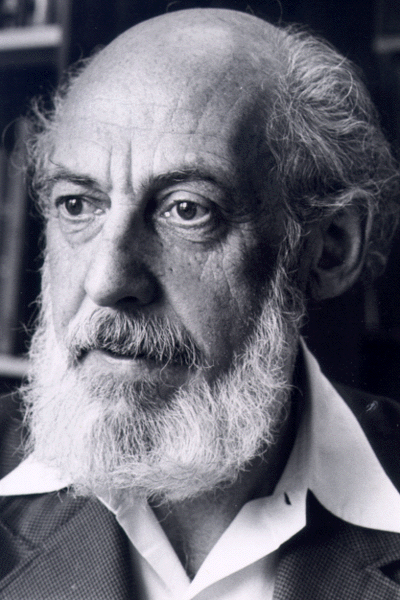
\includegraphics[scale=0.25]{img/Eilenberg.eps}
 \captionsetup{labelformat=empty}
 \caption{艾伦伯格(Samuel Eilenberg, 1913 - 1998)}
 \label{fig:Eilenberg}
\end{wrapfigure}

塞缪尔·艾伦伯格于1913年生于波兰华沙的一个犹太人家庭。他于1936年在华沙大学获得博士学位。艾伦伯格主要研究代数拓扑。他与诺曼·斯廷罗德(Norman Steenrod)一起对同调理论进行了公理化。艾伦伯格在与麦克兰恩合作研究同调代数的过程中一起创立了范畴论。艾伦伯格也是著名的布尔巴基小组成员。他与昂利·嘉当合作,在1956年完成了经典著作《同调代数》。艾伦伯格后来移居美国,在纽约哥伦比亚大学做教授,他的主要工作是发展纯粹的范畴论,是该领域的奠基者之一。1986年他获得沃尔夫奖。1998年艾伦伯格逝世于美国纽约市。

艾伦伯格还是著名的亚洲艺术品收藏家。他收集了来自印度、印度尼西亚、尼泊尔、泰国、柬埔寨、斯里兰卡和中亚的雕塑和艺术品。1992年,他把自己收藏的400多件艺术品捐赠给了纽约大都会博物馆\cite{Wiki-Eilenberg}。

\begin{wrapfigure}{L}{0.3\textwidth}
 \centering
 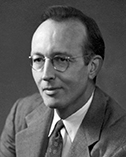
\includegraphics[scale=1]{img/Mac-Lane.eps}
 \captionsetup{labelformat=empty}
 \caption{麦克兰恩(Saunders Mac Lane, 1909 - 2005)}
 \label{fig:Mac-Lane}
\end{wrapfigure}

桑德斯·麦克兰恩1909年生于美国康涅狄格州的诺维奇市。麦克兰恩受洗时的名字是“雷斯利·桑德斯·麦克兰恩”。但是他的父母不喜欢这个名字,所以后来就把雷斯利去掉了。麦克兰恩名字的英文本来是MacLane,他的妻子在打字时总是习惯加上一个空格变成Mac Lane,索性后来麦克兰恩就将错就错了。

麦克兰恩在高中时最喜欢化学。他的父亲在这时去世了,只好由祖父来照顾他。1926年,麦克兰恩的一个远房叔叔资助他到耶鲁学习。他的数学老师希尔带领他参加数学竞赛,并且一路过关斩将获得优胜。从此麦克兰恩下定了从事数学的决心。1930年,麦克兰恩从耶鲁毕业,获得了数学和物理学的双学位。毕业前一年,有一次在新泽西召开耶鲁橄榄球队的球迷聚会。麦克兰恩在会上被授予耶鲁优秀毕业成绩奖\cite{Wiki-Mac-Lane}。恰好芝加哥大学的新任校长哈钦斯也在这次聚会中,他鼓励麦克兰恩到芝加哥大学深造。麦克兰恩于是来到了他后来毕生工作的芝加哥大学\footnote{这里有一段小插曲,聚会后不久,哈钦斯就答应给麦克兰恩一笔奖学金。但是麦克兰恩竟然忘记申请研究生课程就直接去了芝加哥大学。当然最后他被获准入学。}。1931年他获得了硕士学位,接着获得了前往世界数学圣地——哥廷根大学进修的机会。麦克兰恩幸运的成为了最后一批前往哥廷根的美国人,不久纳粹德国就开始禁止美国人前来学习。

在哥廷根,麦克兰恩师从大数学家保罗$\cdot$伯奈斯、埃米$\cdot$诺特、赫尔曼$\cdot$外尔。在他即将获得博士学位的前夕,导师伯奈斯因为是犹太人,被纳粹政府赶出了校园,于是只好由外尔接替伯奈斯。1934年麦克兰恩获得了哥廷根数学研究所的博士学位,并返回美国\footnote{取得学位后,麦克兰恩与来自芝加哥的多萝西$\cdot$琼斯结婚,不久后,他们夫妻一起返回了芝加哥。}。

在1944年与1945年,麦克兰恩领导了在第二次世界大战期间有卓越贡献的哥伦比亚大学应用数学小组。麦克兰恩曾任国家科学院与美国哲学会的副主席,美国数学会的主席。在领导美国数学会的其间,他提倡对现代数学教学技巧改进的研习活动。而在1974年至1980年间,他担任了美国政府的科学顾问。于1976年,以他为首的美国数学家访问团访问了中国,考察了当时中国数学学术发展。麦克兰恩于1949年获选为美国国家科学院院士,并在1989年获得美国国家科学奖章。

麦克兰恩的早期研究方向为域论与赋值论。1941年,麦克兰恩在访问密歇根大学时遇到了艾伦伯格。两人开始在代数和拓扑学上进行合作,并结出了累累硕果。1943年,他与艾伦伯格在研究同调代数时一起创立了范畴论。

2005年,麦克兰恩逝世于美国的旧金山。

\section{范畴}

在介绍范畴的定义前,请先努力忘记集合、函数、映射这些概念。我们以后会看到它们在范畴论中的具体解释。

\begin{definition}
一个范畴$\mathbf{C}$包括一组对象(Object)\footnote{和编程中的“面向对象”无关。这里指抽象事物。},记为$A, B, C, ...$,和一组箭头(Arrow),记为$f, g, h, ...$。它们之上定义了以下四种操作:
\begin{itemize}
\item 两个全操作\footnote{全操作(total operation)是指对于所有的对象,无一例外都存在这一操作。与之相对的是部分操作(partial operation),对于某些对象,这一操作没有定义。例如对于全体整数的集合,取相反数$x \mapsto -x$是全操作,而取倒数$x \mapsto 1/x$由于对0没有定义,所以是部分操作。},称为源(source)和目标(target)\footnote{不应把源和目标理解为名词,而应理解为动词。表示“指定源为……”,“指定目标为……”},这两个操作都将对象指定到箭头上记为$A \xlongrightarrow{f} B$,表示箭头$f$的源是$A$,目标是$B$;
\item 第三个全操作叫恒等箭头\footnote{同样这里恒等箭头(identity arrow)应理解为动词,表示“为……指定恒等箭头”。},对于任何物体$A$,恒等箭头都指向$A$自己。记为:$A \xlongrightarrow{id_A} A$;
\item 第四个操作是一个部分操作,称为组合。它将两个箭头组合起来。如果有箭头$B \xlongrightarrow{f} C$和$A \xlongrightarrow{g} B$,则$f$和$g$的组合为$f \cdot g$,读作“$g$然后$f$”。它表示$A \xlongrightarrow{f \cdot g} C$。
\end{itemize}
\end{definition}

有时我们也将箭头$A \xlongrightarrow{f} B$写成$f: A \to B$,如果上下文中对象很清楚,不会产生歧义,有时也直接简写成$f$。如果将对象简记为$Obj$,箭头简记为$Arw$,则组合操作的类型为$(\cdot) : Arw \times Arw \to Arw$,表示从两个箭头产生一个新的箭头;源的类型为$src: Arw \to Obj$,表示为某一箭头指定源;目标的类型为$trg: Arw \to Obj$,为某一箭头指定目标;恒等箭头的类型为$id: Obj \to Arw$,表示为某一对象指定恒等箭头。



\section{函子}

\section{自然变换}

\section{积和余积}

\section{数据类型}

\section{伴随}

\ifx\wholebook\relax \else
\begin{thebibliography}{99}

\bibitem{Dieudonne1987}
[法]让$\cdot$迪厄多内 著,沈用欢 译 ``当代数学,为了人类心智的荣耀''. 上海教育出版社. 2000年3月. ISBN: 7532063062

\bibitem{Monad-Haskell-Wiki}
Haskell Wiki. ``Monad''. \url{https://wiki.haskell.org/Monad}

\bibitem{Wiki-Eilenberg}
Wikipedia. ``塞缪尔$\cdot$艾伦伯格''. \url{https://en.wikipedia.org/wiki/Samuel_Eilenberg}

\bibitem{Wiki-Mac-Lane}
Wikipedia. ``桑德斯$\cdot$麦克兰恩''. \url{https://en.wikipedia.org/wiki/Saunders_Mac_Lane}

\end{thebibliography}

\expandafter\enddocument
%\end{document}

\fi
